\let\negmedspace\undefined
\let\negthickspace\undefined
\documentclass[journal]{IEEEtran}
\usepackage[a5paper, margin=10mm, onecolumn]{geometry}
%\usepackage{lmodern} % Ensure lmodern is loaded for pdflatex
\usepackage{tfrupee} % Include tfrupee package

\setlength{\headheight}{1cm} % Set the height of the header box
\setlength{\headsep}{0mm}     % Set the distance between the header box and the top of the text

\usepackage{gvv-book}
\usepackage{gvv}
\usepackage{cite}
\usepackage{amsmath,amssymb,amsfonts,amsthm}
\usepackage{algorithmic}
\usepackage{graphicx}
\usepackage{textcomp}
\usepackage{xcolor}
\usepackage{txfonts}
\usepackage{listings}
\usepackage{enumitem}
\usepackage{mathtools}
\usepackage{gensymb}
\usepackage{comment}
\usepackage[breaklinks=true]{hyperref}
\usepackage{tkz-euclide}
\usepackage{listings}                                     
\def\inputGnumericTable{}                                 
\usepackage[utf8]{inputenc}                                
\usepackage{color}                                            
\usepackage{array}                                            
\usepackage{longtable}                                       
\usepackage{calc}                                             
\usepackage{multirow}                                         
\usepackage{hhline}                                           
\usepackage{ifthen}                                           
\usepackage{lscape}
\renewcommand{\thefigure}{\theenumi}
\renewcommand{\thetable}{\theenumi}
\setlength{\intextsep}{10pt} % Space between text and floats

\numberwithin{equation}{enumi}
\numberwithin{figure}{enumi}
\renewcommand{\thetable}{\theenumi}

% Marks the beginning of the document
\begin{document}
\bibliographystyle{IEEEtran}

\title{Question-3.4.2.3}
\author{EE24BTECH11048-NITHIN.K} 
%\maketitle
%\newpage
%\bigskip
{\let\newpage\relax\maketitle}
\textbf{Question:}\\
The sum of the two digits of a two-digit number is 9. Also nine times this number is twice the number obtained by reversing the order of the digits.\\
\textbf{Theoretical Solution:}\\
\begin{align}
	x + y &= 9\\
	9\brak{10x + y} &= 2\brak{10y + x}\\
	8x - y &= 0
\end{align}
The system of linear equations can be written as:
\begin{align}
	A\vec{x} = \vec{b}
\end{align}
where
\begin{align}
	A = \myvec{1 & 1\\
	8 & -1},\quad \vec{x} = \myvec{x\\y},\quad \vec{b} = \myvec{9\\0}
\end{align}
\textbf{Dolittle's Algorithm:}\\
The LU decomposition splits $A$ into a lower triangular matrix $L$ and an upper triangular matrix $U$ such that:\\
\begin{align}
	A = LU
\end{align}
Where:\\
\begin{align}
	L = \myvec{1 & 0 & 0 & \cdots & 0 \\ L_{21} & 1 & 0 & \cdots & 0 \\ L_{31} & L_{32} & 1 & \cdots & 0 \\ \vdots & \vdots & \vdots & \ddots & 0 \\ L_{n1} & L_{n2} & L_{n3} & \cdots & 1},\quad
	U = \myvec{U_{11} & U_{12} & U_{13} & \cdots & U_{1n} \\ 0 & U_{22} & U_{23} & \cdots & U_{2n} \\ 0 & 0 & U_{33} & \cdots & U_{3n} \\ \vdots & \vdots & \vdots & \ddots & U_{n-1,n} \\ 0 & 0 & 0 & \cdots & U_{nn}}.
\end{align}
The Doolittle algorithm is computed as follows:\\
Elements of the $U$ Matrix: \\  
For each column $j $:
\begin{align}
	U_{ij} = A_{ij} \text{ if } i = 0,\\
	U_{ij} = A_{ij} - \sum_{k=0}^{i-1} L_{ik} U_{kj} \text{ if } i > 0.
\end{align}
Elements of the $L$ Matrix:\\  
For each row $i $:  
\begin{align}
	L_{ij} = \frac{A_{ij}}{U_{jj}} \text{ if } j = 0, \\  
	L_{ij} = \frac{A_{ij} - \sum_{k=0}^{j-1} L_{ik} U_{kj}}{U_{jj}} \text{ if } j > 0.  
\end{align}
Performing LU Decomposition using Dolittle's Algorithm, we get:
\begin{align}
	L = \myvec{1 & 0\\
	8 & 1}, \quad U = \myvec{1 & 1\\
	0 & -9}
\end{align}
Now we solve the system in two steps using forward substitution and backward substitution.\\
First Solve $L\vec{y} = \vec{b}$ for $\vec{y}$ :
\begin{align}
	\myvec{1 & 0\\8 & 1}\myvec{y_1\\y_2} = \myvec{9\\0}
\end{align}
\begin{align}
	y_1 = 9
\end{align}
\begin{align}
	8y_1 + y_2 = 0, \quad y_2 = -72
\end{align}
\begin{align}
	\vec{y} =  \myvec{9\\-72}
\end{align}
Solve for $U\vec{x} = \vec{y}$ for $\vec{x}$ :
\begin{align}
	\myvec{1 & 1\\0 & -9}\myvec{x\\y} = \myvec{9\\-72}
\end{align}
\begin{align}
        -9y = -72, \quad y = 8
\end{align}
\begin{align}
	x + y = 9
\end{align}
\begin{align}
	x = 1
\end{align}
Thus the solution is $x = 1, y = 8$

\begin{figure}[H]
    \centering
    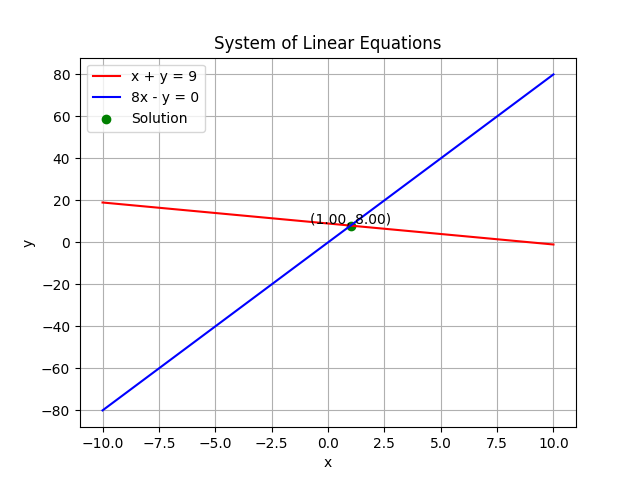
\includegraphics[width=\textwidth]{figs/fig.png}
\end{figure}

\end{document}
